\documentclass[11pt,a4paper]{article}

\usepackage[utf8]{inputenc}
\usepackage{url}
\usepackage[margin=1in]{geometry}
\usepackage{graphicx}

\title{GitHub Cheat Sheet}
\date{}
\author{Econ 213R - Applied Machine Learning}

\begin{document}
\vspace*{-75pt}
    {\let\newpage\relax\maketitle}
    
\section*{What is GitHub?}
\begin{itemize}
\item Explain idea of GitHub
\item Define ``repository"
\item Define ``fork", ``clone", ``commit", ``push/pull"
\item Explain what a README is
\end{itemize}
    
\section*{Register for GitHub}
First, you need to make an account with GitHub.
Go to \url{www.github.com}. 
Sign up from the home page with any email and username you want.
Follow the initial signup steps.
Note that private repositories require monthly payments; however, you can have an unlimited number of public repositories for free.
Once you are done signing up, you are ready to create and fork repositories.

\section*{Creating Repositories}
Navigate to your GitHub profile.
It should look something like Figure \ref{fig:init-prof}.

\begin{figure}[h]
\centering
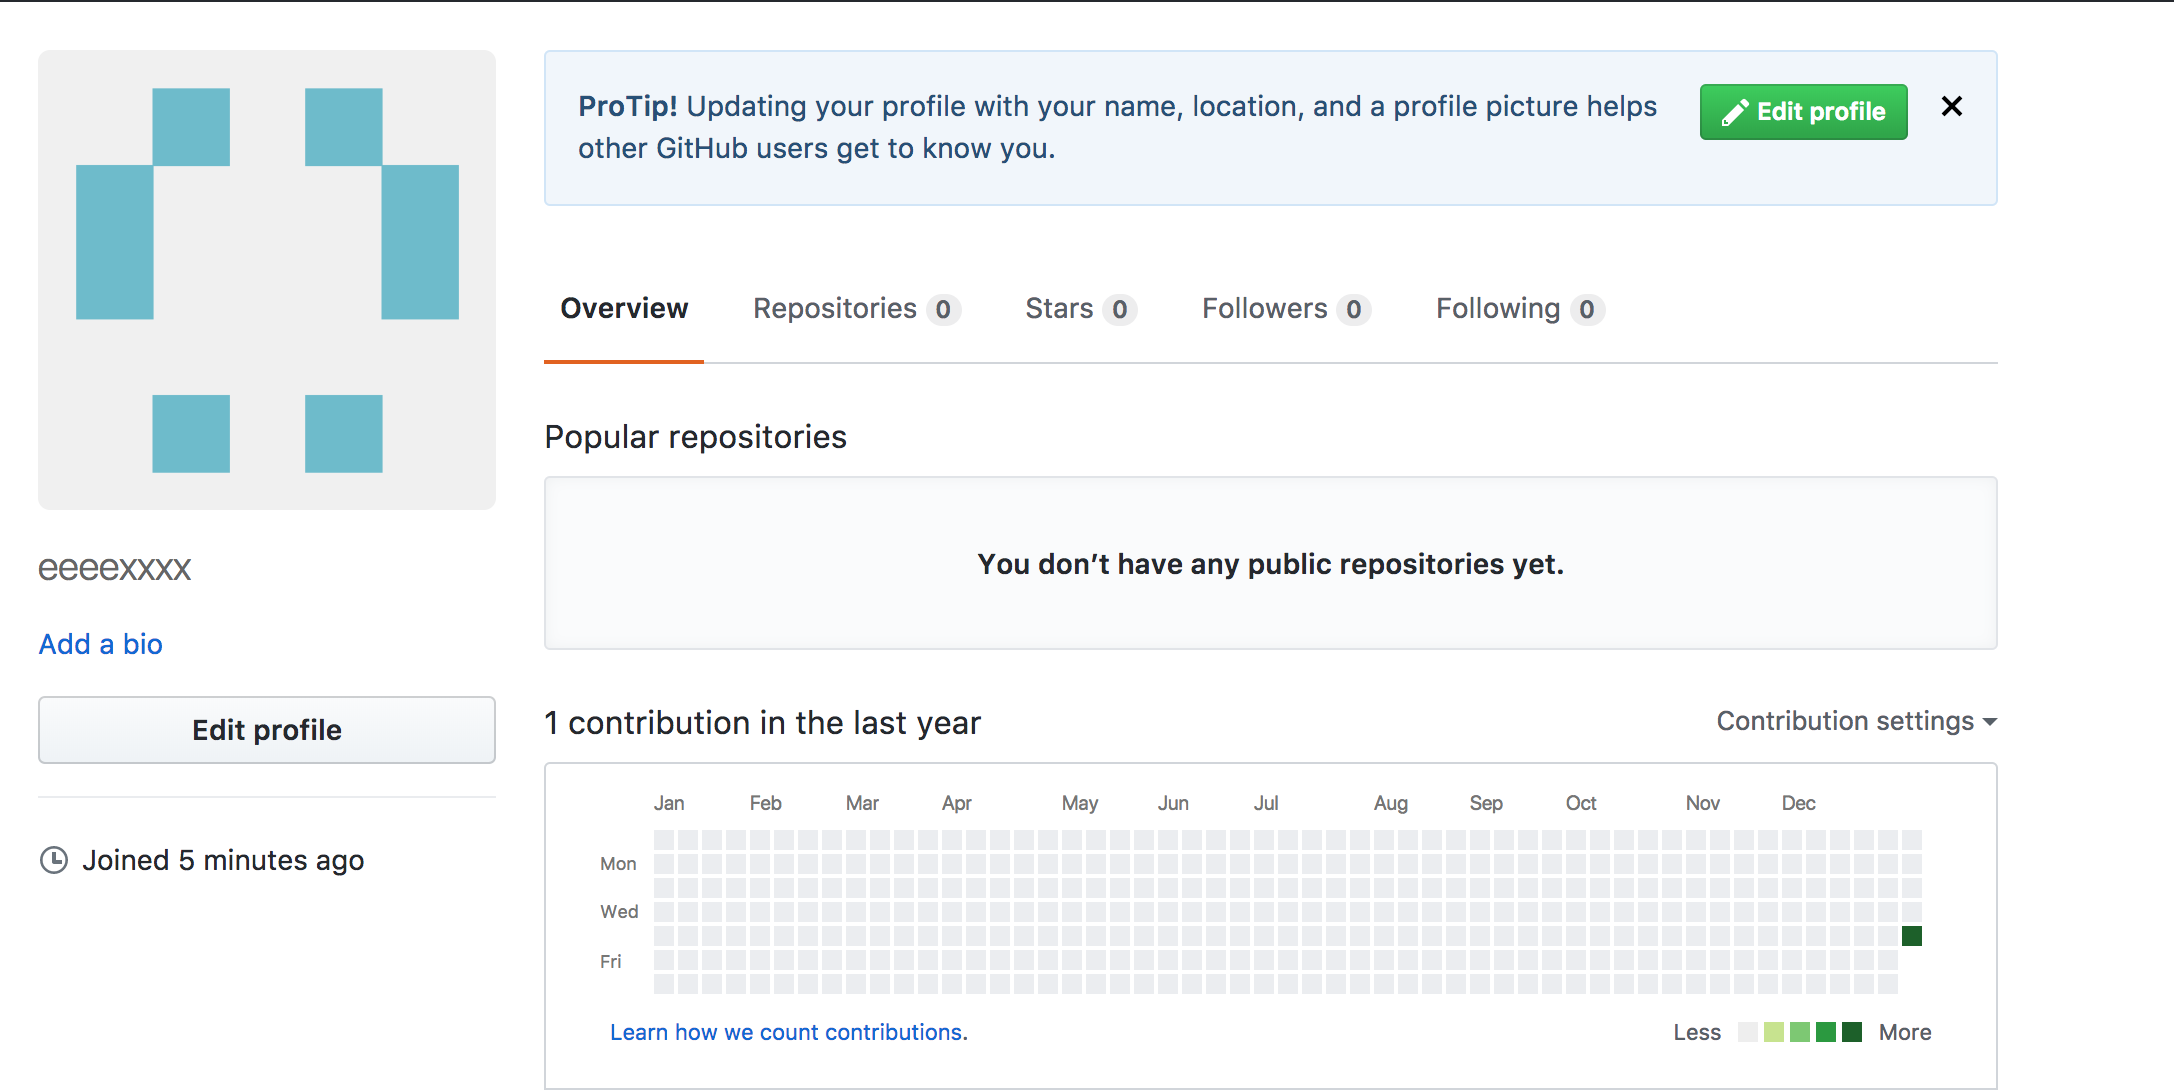
\includegraphics[width=.7\textwidth]{figures/init_profile.png}
\caption{Profile Screen}
\label{fig:init-prof}
\end{figure}

Click the ``Repositories" tab.
Click the button that says ``New" (see Figure \ref{fig:repo}).

\begin{figure}[h]
\centering
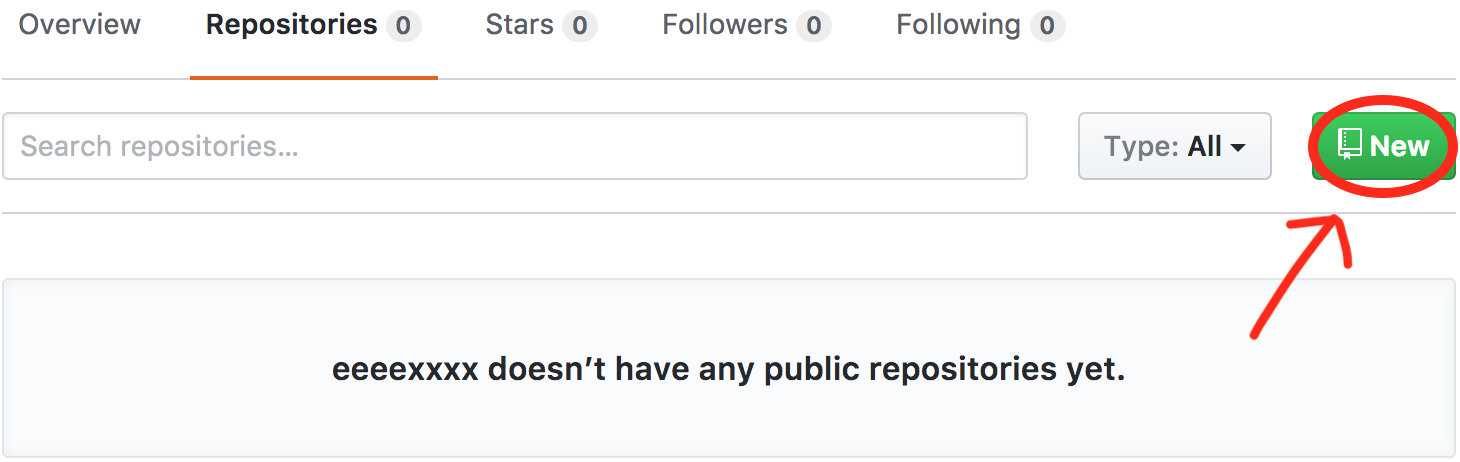
\includegraphics[width=.7\textwidth]{figures/repository_page.png}
\caption{Repository Screen}
\label{fig:repo}
\end{figure}

Name your repository.
It is customary to use dashes instead of underscores in repository names.
Make sure to initialize the repository with a README.md (see Figure \ref{fig:init-repo}).
If you accidentally forget to do this, that's okay; you can always add a README later.

\begin{figure}[h]
\centering
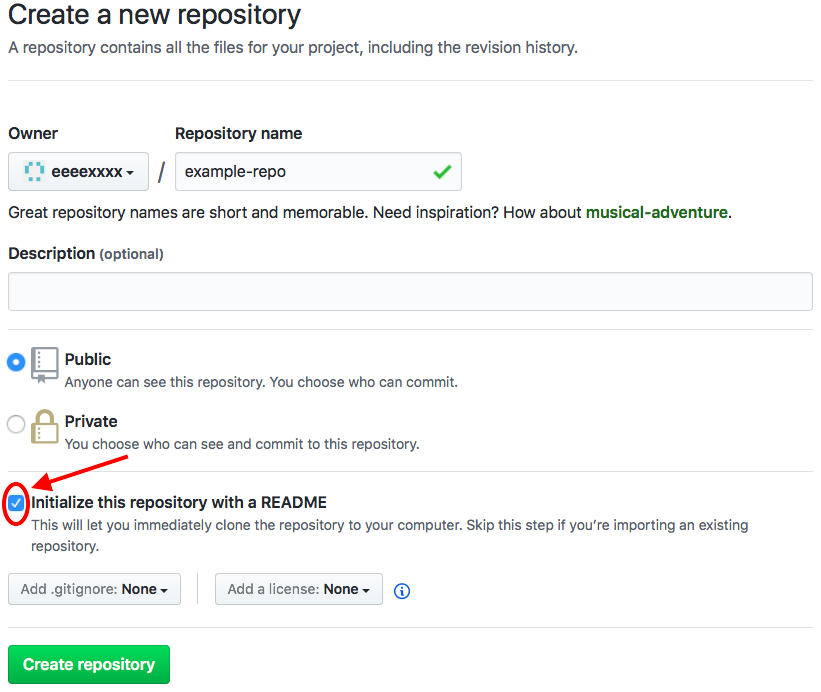
\includegraphics[width=.7\textwidth]{figures/init_repo}
\caption{Initialize the repository.}
\label{fig:init-repo}
\end{figure}

Click ``Create Repository" at the bottom of the page.
Congratulations!
You have just created your first GitHub repository.

\section*{Making Changes to Repositories}
There are a few ways to upload and change files in a GitHub repository.
The most common way to modify repositories is via the command line; see the next subsection for command line instructions.
It is highly, \textit{highly} recommended that you learn the command line to modify repositories.
The command line allows you to more freedom to modify your repositories and branches, and can streamline your workflow.
However, you can use the GitHub website to upload and download files to and from repositories.
You can also modify files using the website.
Note that you can't run Jupyter notebooks on the GitHub website, and when you try to edit Jupyter notebooks on the website, you have to comb through lots of nasty JSON lingo.
If you choose to use the website to make changes to the GitHub repository, you will have to download the Jupyter notebook, modify it on a local machine, and upload it back to the repository.
Instructions for using the website are in the subsection following the command line instructions.

\subsection*{Using Command Line}
\subsubsection*{Making Changes}

\subsubsection*{Committing Changes}

\subsubsection*{Pulling Changes}

\subsection*{Using the Website}
\subsubsection*{Downloading Files}

\subsubsection*{Uploading Files}

\section*{Forking Repositories}
Navigate to the class repository. 
The link is \url{https://github.com/tfolkman/byu_econ_applied_machine_learning}.

\end{document}